%%=============================================================================
%% Methodologie
%%=============================================================================

\chapter{Methodologie}
\label{ch:methodologie}

%% TODO: Hoe ben je te werk gegaan? Verdeel je onderzoek in grote fasen, en
%% licht in elke fase toe welke stappen je gevolgd hebt. Verantwoord waarom je
%% op deze manier te werk gegaan bent. Je moet kunnen aantonen dat je de best
%% mogelijke manier toegepast hebt om een antwoord te vinden op de
%% onderzoeksvraag.

\section{Creatie proof-of-concept foto-app}
\label{sec:proofofconcept}

Om het onderzoek te onderbouwen, werd een Android Wear proof-of-concept app gecreërd. Dit is een algemene applicatie, waarin verschillende elementen toegevoegd worden zoals media-bestanden, veel code.. Het doel van de creatie van deze app is om de verschillende compressietechnieken hierop toe te passen, en de resultaten grafisch voor te stellen. De applicatie draait op Android Wear 2.0, deze versie werd op 09/02/2017 uitgebracht door Google.\autocite{Google} Doordat voor deze versie gekozen werd, kan de app als standalone app gebruikt worden. Dit houdt in dat de app op een smartwatch kan gebruikt worden onafhankelijk van een smartphone. De gebruikers kunnen meer taken op hun smartwatch uitvoeren zonder toegang tot een Android of iOS smartphone. De app zal als functie hebben om gemakkelijk notities te maken via spraakherkenningstechnologie. Hierdoor kunnen de gebruikers door te spreken in de microfoon van de smartwatch een nieuwe notitie maken. Deze notities worden dan weergeven in een tabel die weergeven wordt wanneer een notitie werd toegevoegd. Voor elk scherm van de app werd een andere achtergrondafbeelding gebruikt om zo de compressie van afbeeldingen achteraf beter te kunnen testen. Op deze afbeeldingen werd vooraf nog geen compressie toegepast, er werden afbeeldingen van een standaardgrootte gebruikt die dan automatisch gescaled werden naar de grootte van de image views. In de app zit ook een splashscreen (scherm dat weergeven wordt tijdens het opstarten van de applicatie) verwerkt. 
\begin{figure}[H]
	\centering
	\caption{\textit{Hoofdscherm foto-app}}
	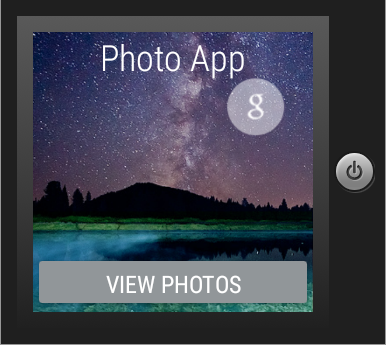
\includegraphics[width=7cm, height=7cm, keepaspectratio]{img/photoappmain}\\[.5cm]
\end{figure}
\begin{figure}[H]
	\centering
	\caption{\textit{Foto view}}
	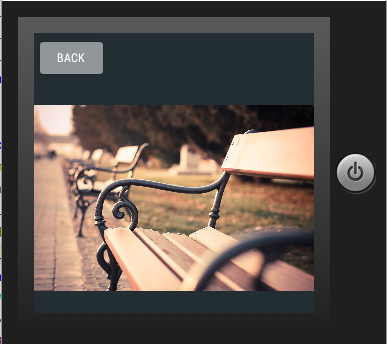
\includegraphics[width=7cm, height=7cm, keepaspectratio]{img/photoappgallery}\\[.5cm]
	
\end{figure}

\section{Verschillende technieken toepassen op proof-of-concept app}
\label{sec:techniekentoepassen}


\section{Prestaties en grootte app testen na toepassen technieken}
\label{sec:prestatiesgrootteapp}

\section{Testen van app door framework Brian Pinsard}
\label{sec:apptesting}